\chapter{Finite State Machines}\label{ch12}
\section{Introduction}


%***************************************************************************
% Section: Finite State Machines
%***************************************************************************
\section{Finite State Machines}
\label{SIM:sec:finite_state_machines}

\subsection{Introduction}
\label{SIM:subsec:intro_to_finite_state_machines}

Sequential logic circuits are dynamic and the combined inputs and outputs of the circuit at any given stable moment is called a \emph{state}. Over time, a circuit changes states as triggering events take place. As an example, a traffic signal may be green at some point but change to red because a pedestrian presses the  ``cross'' button. The current state of the system would be ``green'' but the triggering event (the ``cross'' button) changes the state to ``red.'' 

The mathematical model of a sequential circuit is called a \gls{fsm}. A \gls{fsm} is an abstract model of a sequential circuit where each state of the circuit is indicated by circles and various triggering events are used to sequence a process from one state to the next. The behavior of many devices can be represented by a \gls{fsm} model, including traffic signals, elevators, vending machines, and robotic devices. \glspl{fsm} are an analysis tool that can help to simplify sequential circuits. 

There are two fundamental \gls{fsm} models: Moore and Mealy. These two models are generalizations of a state machine and differ only in the way that the outputs are generated. A Moore machine generates an output as a function of only the current state while a Mealy machine generates an output as a function of the current state plus the inputs into that state. Moore machines tend to be safer since they are only activated on a clock pulse and are less likely to create unwanted feedback when two different modules are interconnected; however, Mealy machines tend to be simpler and have fewer states than a Moore machine. Despite the strengths and weaknesses for each of these two \glspl{fsm}, in reality, they are so similar that either can be effectively used to model any given circuit and the actual \gls{fsm} chosen by the designer is often little more than personal preference. 

\subsection{Moore Finite State Machine}
\label{SIM:subsec:moore_finite_state_machine}

The Moore \gls{fsm} is named after Edward F. Moore, who presented the concept in a $ 1956 $ paper, \emph{Gedanken-experiments on Sequential Machines}. The output of a Moore \gls{fsm} depends only on its current state. The Moore \gls{fsm} is typically simpler than a Mealy \gls{fsm} so modeling hardware systems is usually best done using a Moore \gls{fsm}. 

As an example of a Moore \gls{fsm} imagine a simple candy vending machine that accepts either five cents or ten cents at a time and vends a handful of product when $ 15 $ cents has been deposited (no change is returned). Figure \ref{SIM:fig:moore_vending_machine_fsm} is a Moore \gls{fsm} diagram for this vending machine.

\begin{figure}[H]
  \caption{Moore Vending Machine FSM}
  \label{SIM:fig:moore_vending_machine_fsm}
  \myfloatalign
  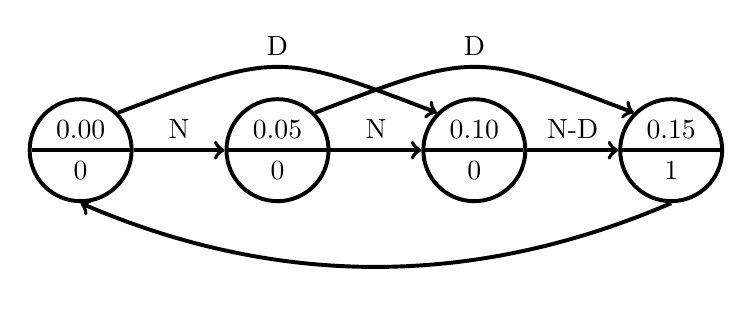
\begin{tikzpicture} [scale=1.00]
  \usepgflibrary{shapes.multipart} % for the multipart nodes
  % make all path lines (the node shapes) a little thicker
  \tikzstyle{every path}=[line width=0.50mm]  
  
  % Draw the lines
  \node [circle split,draw] (00) at (2.00, 4) {$ 0.00 $ \nodepart{lower} $ 0 $};
  \node [circle split,draw] (05) at (4.50, 4) {$ 0.05 $ \nodepart{lower} $ 0 $};
  \node [circle split,draw] (10) at (7.00, 4) {$ 0.10 $ \nodepart{lower} $ 0 $};
  \node [circle split,draw] (15) at (9.50, 4) {$ 0.15 $ \nodepart{lower} $ 1 $};
  
  % ``N'' Arrows
  \draw[->] (00.east) .. controls (3.25,4)  .. node[above] {N} (05.west);
  \draw[->] (05.east) .. controls (5.75,4)  .. node[above] {N} (10.west);
  \draw[->] (10.east) .. controls (8.25,4)  .. node[above] {N-D} (15.west);
  
  % ``D'' Arrows
  \draw[->] (00.north east) .. controls (4.50,5.25)  .. node[above] {D} (10.north west);
  \draw[->] (05.north east) .. controls (7.00,5.25)  .. node[above] {D} (15.north west);
  
  % ``Vend'' Arrow
  \draw[->] (15.south) .. controls (7.00,2.25) and (4.50,2.25)  .. node[below] {} (00.south);  
  ;
  \end{tikzpicture}
\end{figure}

In Figure \ref{SIM:fig:moore_vending_machine_fsm}, imagine that five cents is deposited between each state circle (that action is indicated by the arrows labeled with an $ N $, for Nickel). The output at each state is zero (printed at the bottom of each circle) until the state reaches $ 0.15 $ in the last circle, then the output changes to one (the product is vended). After that state is reached the system resets to state $ 0.00 $ and the entire process starts over. If a user deposits ten cents, a Dime, then one of the nickel states is skipped.

\subsection{Mealy Finite State Machine}
\label{SIM:subsec:mealy_finite_state_machines}

The Mealy machine is named after George H. Mealy, who presented the concept in a $ 1955 $ paper, \emph{A Method for Synthesizing Sequential Circuits}. The Mealy \gls{fsm} output depends on both its current state and the inputs. Typically a Mealy machine will have fewer states than a Moore machine, but the logic to move from state to state is more complex. 

As an example of a Mealy \gls{fsm}, the simple candy vending machine introduced in Figure \ref{SIM:fig:moore_vending_machine_fsm} can be redesigned. Recall that the machine accepts either five cents or ten cents at a time and vends a handful of product when $ 15 $ cents has been deposited (no change is returned). Figure \ref{SIM:fig:mealy_vending_machine_fsm} is a Mealy \gls{fsm} diagram for this vending machine.

\begin{figure}[H]
  \caption{Mealy Vending Machine FSM}
  \label{SIM:fig:mealy_vending_machine_fsm}
  \myfloatalign
  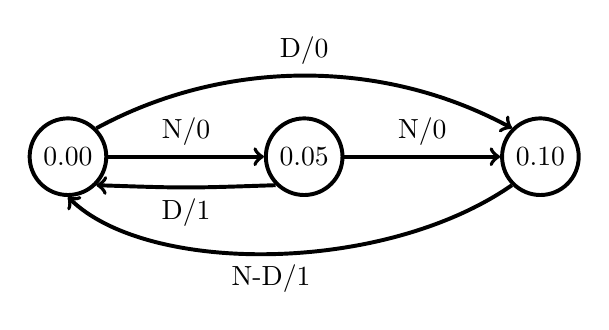
\begin{tikzpicture} [scale=1.00]
  \usepgflibrary{shapes.multipart} % for the multipart nodes
  % make all path lines (the node shapes) a little thicker
  \tikzstyle{every path}=[line width=0.50mm]  
  
  % Draw the lines
  \node [circle,draw] (00) at (2.00, 4) {$ 0.00 $};
  \node [circle,draw] (05) at (5.00, 4) {$ 0.05 $};
  \node [circle,draw] (10) at (8.00, 4) {$ 0.10 $};
  %  \node [circle,draw] (15) at (9.50, 4) {$ 0.15 $};
  
  % ``N'' Arrows
  \draw[->] (00.east) .. controls (3.50,4)  .. node[above] {N/$0$} (05.west);
  \draw[->] (05.east) .. controls (6.50,4)  .. node[above] {N/$0$} (10.west);
  
  % ``D'' Arrows
  \draw[->] (00.north east) .. controls (4.00,5.25) and (6.00,5.25)  .. node[above] {D/$0$} (10.north west);
  \draw[->] (05.south west) .. controls (3.50,3.60)  .. node[below] {D/$1$} (00.south east);
  
  % ``Vend'' Arrow
  \draw[->] (10.south west) .. controls (6.00,2.50) and (3.00,2.50)  .. node[below] {N-D/$1$} (00.south);  
  ;
  \end{tikzpicture}
\end{figure}

In Figure \ref{SIM:fig:mealy_vending_machine_fsm} the states are identified by the amount of money that has been deposited, so the first state on the left ($ 0.00 $) is when no money has been deposited. Following the path directly to the right of the first state, if five cents (indicated by ``N'' for a nickel) is deposited, then the output is zero (no candy is dispensed) and the state is changed to $ 0.05 $. If another five cents is deposited, the output remains zero and the state changes to $ 0.10 $. At that point, if either five or ten cents (``N'' or ``D'') is deposited, then the output changes to $ 1 $ (candy is dispensed) and the state resets to $ 0.00 $. By following the transition arrows various combinations of inputs and their resulting output can be traced.

Because the Mealy \gls{fsm} reacts immediately to any input it requires one less state than the Moore machine (compare Figures \ref{SIM:fig:moore_vending_machine_fsm} and \ref{SIM:fig:mealy_vending_machine_fsm}). However, since Moore machines only change states on a clock pulse they tend to be more predictable (and safer) when integrated into other modules. Finally, Mealy machines tend to react faster than Moore machines since they do not need to wait for a clock pulse and, generally, are implemented with fewer gates. In the end, whether to design with a Mealy or a Moore machine is left to the designer's discretion and, practically speaking, most designers tend to favor one type of \gls{fsm} over the other. The simulations in this book use Moore machines because they tend to be easier to understand and more stable in operation.

\subsection{Finite State Machine Tables}
\label{SIM:subsec:finite_state_machine_tables}

Many designers enjoy using Moore and Mealy \gls{fsm} diagrams as presented in Figures \ref{SIM:fig:moore_vending_machine_fsm} and \ref{SIM:fig:mealy_vending_machine_fsm}; however, others prefer to design with a finite state machine table that lists all states, inputs, and outputs. As an example, imagine a pedestrian crosswalk in the middle of a downtown block. The crosswalk has a traffic signal to stop traffic and a \emph{Cross / Don't Cross} light for pedestrians. It also has a button that pedestrians can press to make the light change so it is safe to cross.

This system has several states which can be represented in a \emph{State Table}. The traffic signal can be Red, Yellow, or Green and the pedestrian signal can be Walk or Don't Walk. Each of these signals can be either zero (for \emph{Off}) or one (for \emph{On}). Also, there are two triggers for the circuit; a push button (the \emph{Cross} button that a pedestrian presses) and a timer (so the walk light will eventually change to don't walk). If the button is assumed to be one when it is pressed and zero when not pressed, and the timer is assumed to be one when a certain time interval has expired but zero otherwise, then State Table \ref{SIM:tab:crosswalk_state_table} can be created.

\begin{table}[H]
  \sffamily
  \newcommand{\head}[1]{\textcolor{white}{\textbf{#1}}}    
  \begin{center}
    \rowcolors{2}{gray!10}{white} % Color every other line a light gray
    \begin{tabular}{ccccccccccccc} 
      \rowcolor{black!75}
      & \multicolumn{5}{c}{\head{Current State}} & \multicolumn{2}{c}{\head{Trigger}} & \multicolumn{5}{c}{\head{Next State}} \\
      & R & Y & G & W & D & Btn & Tmr & R & Y & G & W & D \\
      \hline
      1 & 0 & 0 & 1 & 0 & 1 & 0 & 0 & 0 & 0 & 1 & 0 & 1 \\
      2 & 0 & 0 & 1 & 0 & 1 & 1 & 0 & 0 & 1 & 0 & 0 & 1 \\
      3 & 0 & 1 & 0 & 0 & 1 & X & 0 & 1 & 0 & 0 & 1 & 0 \\
      4 & 1 & 0 & 0 & 1 & 0 & X & 1 & 0 & 0 & 1 & 0 & 1
    \end{tabular}
  \end{center}
  \caption{Crosswalk State Table}
  \label{SIM:tab:crosswalk_state_table}
\end{table}

The various states are $ R $ (for \emph{Red}), $ Y $ (for \emph{Yellow}), and $ G $ (for \emph{Green}) traffic lights, and $ W $ (for \emph{Walk}) and $ D $ (for \emph{Don't Walk}) pedestrian lights. The \emph{Btn} (for \emph{Cross Button}) and \emph{Tmr} (for \emph{Timer}) triggers can, potentially, change the state of the system. 

Row One on this table shows that the traffic light is Green and the pedestrian light is Don't Walk. If the button is not pressed (it is zero) and the timer is not active (it is zero), then the next state is still a Green traffic light and Don't Walk pedestrian light; in other words, the system is quiescent. In Row Two, the button was pressed (\emph{Btn} is one); notice that the traffic light changes state to Yellow, but the pedestrian light is still Don't Walk. In Row Three, the current state is a Yellow traffic light with Don't Walk pedestrian light (in other words, the \emph{Next State} from Row Two), the $ X $ for the button means it does not matter if it is pressed or not, and the next state is a Red traffic light and Walk pedestrian light. In Row Four, the timer expires (it changes to one at the end of the timing cycle), and the traffic light changes back to Green while the pedestrian light changes to Don't Walk. 

While Table \ref{SIM:tab:crosswalk_state_table} represents a simplified traffic light system, it could be extended to cover all possible states. Since Red, Yellow, and Green can never all be one at one time, nor could Walk and Don't Walk, the designer must specifically define all of the states rather than use a simple binary count from $ 00000 $ to $ 11111 $. Also, the designer must be certain that some combinations never happen, like a Green traffic light and a Walk pedestrian light at the same time, so those must be carefully avoided. 

State tables can be used with either Mealy or Moore machines and a designer could create a circuit that would meet all of the requirements from the state table and then realize that circuit to actually build a traffic light system. 

